\section{Certified Results}
\label{sec:results}

This section reports only values bound to the checked-in certificate.  The
primary metric is the compiled CNOT upper bound; merged fragment
exponentials and bond propagators are reported because they make the integer
cost model transparent.

\subsection{Headline resource reduction}

The current D5-integrated certificate accepts $r=95$ steps.  Adjacent
identical fragment exponentials merge across recursive boundaries, so a
31-stage step sequence contains
\begin{equation}
  G(r)=30r+1
  \label{eq:merged-groups}
\end{equation}
merged group exponentials.  Each group is one perfect matching with 72 bonds.
The selected two-qubit bond-propagator compilation is charged at three CNOTs.
Therefore
\begin{equation}
  B(r)=72G(r),\qquad C(r)=3B(r)=216G(r).
  \label{eq:resource-map}
\end{equation}

\begin{table}[t]
\centering
\caption{Certified resource comparison under the common compilation model.}
\label{tab:headline-results}
\begin{tabular}{@{}lrrrr@{}}
\toprule
Method & Steps & Merged groups & Bond propagators & CNOT upper \\
\midrule
Pinned published-theorem control & 393 & 11,791 & 848,952 & 2,546,856 \\
Proof-carrying model-aware bound & 95 & 2,851 & 205,272 & 615,816 \\
\midrule
Candidate/control & 0.2417 & 0.2418 & 0.2418 & 0.2418 \\
\bottomrule
\end{tabular}
\end{table}

Because the last three resource measures are proportional under
\cref{eq:resource-map}, their exact improvement factor is
\begin{equation}
  \frac{11{,}791}{2{,}851}=4.135741844966678\ldots.
  \label{eq:exact-ratio}
\end{equation}
Equivalently, 8,940 of 11,791 merged groups are removed, a reduction of
75.82054109066237\%.  The claimed multiplier is an exact rational comparison;
the decimal is for readability.

\begin{figure}[t]
  \centering
  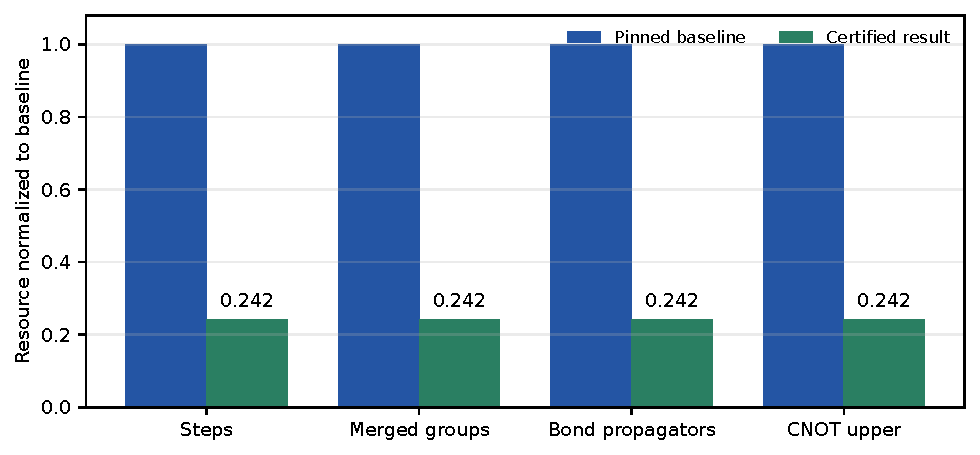
\includegraphics[width=0.94\textwidth]{figures/resources.pdf}
  \caption{Resources for the pinned theorem instantiation and the certified
  model-aware result.  Values are exact integers; axes are scaled separately
  to keep the three compiled metrics readable.}
  \label{fig:resources}
\end{figure}

\subsection{Finite-step error ledger}

At 95 steps the global upper bound is the sum of five outward rational
contributions shown in \cref{tab:error-ledger}.  The leading D4 term is only
57.77\% of the final value; D5--D7 and the tail are quantitatively material.
This demonstrates why a leading-order-only prediction would not be an
adequate certificate at the boundary.

\begin{table}[t]
\centering
\caption{Outward decimal summaries of exact rational contributions at
$r=95$.}
\label{tab:error-ledger}
\begin{tabular}{@{}lrr@{}}
\toprule
Contribution & Global error upper & Fraction of total (approx.) \\
\midrule
D4 & $5.721880076013265\times10^{-7}$ & 57.77\% \\
D5 & $3.485348461510363\times10^{-8}$ & 3.52\% \\
D6 & $1.789314087745318\times10^{-7}$ & 18.07\% \\
D7 & $2.192136130355397\times10^{-8}$ & 2.21\% \\
Tail & $1.825548779887292\times10^{-7}$ & 18.43\% \\
\midrule
Total & $9.904491402832451\times10^{-7}$ & 100\% \\
\bottomrule
\end{tabular}
\end{table}

\begin{figure}[t]
  \centering
  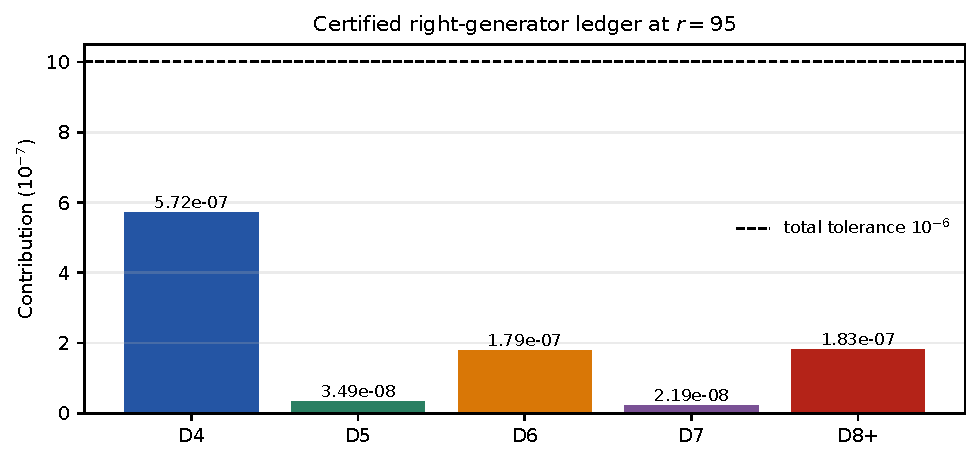
\includegraphics[width=0.72\textwidth]{figures/error_ledger.pdf}
  \caption{Finite-step error ledger at the accepted integer.  The dashed line
  marks the total tolerance, not an independent allowance for each term.}
  \label{fig:error-ledger}
\end{figure}

The adjacent-step evidence is decisive for the integer search:
95 is accepted at $9.904491402832451\times10^{-7}$, whereas the same bound at
94 evaluates to $1.046806116560371\times10^{-6}$.  The margin at 95 is about
$9.55\times10^{-9}$, so outward arithmetic and tail closure are not cosmetic;
ordinary double-precision summaries are not the source of the comparison.

\subsection{Algebraic compression statistics}

The D4 group sidecar contains 75,324 coefficient-bearing Pauli terms divided
into 7,576 verified groups.  The largest group has ten members.  The grouped
translation-cell norm $6.472926505087888$ replaces a post-aggregation direct
Pauli-$\ell_1$ value $20.160968407335066$, giving the local factor
$3.114660484942633$.  This local factor and the final resource factor need not
coincide: the latter also reflects the nonlinear inversion of the step bound,
the subleading terms, the tail, and the integer merge rule.

The integrated exact D5 computation produces 605,832 terms, 123,106 groups,
and the per-site upper bound $11.23706750025697$.  Replacing the predecessor's
generic D5 majorant by this hash-bound grouped witness is the change that moves
the certified boundary from 97/96 to 95/94.  The D4 witness, product formula,
benchmark, tail construction, and compilation rule are unchanged.

\subsection{Small-system structural cross-check}

On a nondegenerate open $2\times3$ instance with seven unique bonds, direct
dense evaluation of the same 95-step stage sequence gives operator-norm error
$1.8313133889571672\times10^{-10}$.  A deliberately outward, size-scaled
periodic-certificate comparison is $4.129166666666667\times10^{-8}$ and
dominates the observation.  This diagnostic checks stage order, normalization,
and nontrivial bond bookkeeping using a dense route independent of the Pauli
certificate.  Because it changes the boundary condition and uses a scaled
comparison rather than an open-boundary theorem, it is not an empirical proof
of the $12\times12$ result.

\subsection{Recursive Suzuki audit}

For context, the D5-integrated certificate carries forward a separate audit of
standard recursive Suzuki orders under its declared audit assumptions.  The
values in \cref{tab:recursive-audit} are taken from that manifest-bound
schema-v3 JSON; they are not used in the primary 4.1357$\times$ comparison.

\begin{table}[t]
\centering
\caption{Auxiliary recursive-order audit stored in the current certificate.}
\label{tab:recursive-audit}
\begin{tabular}{@{}rrrrr@{}}
\toprule
Order & Steps & Stages/step & Merged groups & Error upper summary \\
\midrule
2 & 29,964 & 7 & 179,785 & $9.9999203748666826\times10^{-7}$ \\
4 & 808 & 31 & 24,241 & $9.9682621337975879\times10^{-7}$ \\
6 & 370 & 151 & 55,501 & $9.8463753882538689\times10^{-7}$ \\
8 & 335 & 751 & 251,251 & $9.9829085642259163\times10^{-7}$ \\
\bottomrule
\end{tabular}
\end{table}

This audit illustrates that increasing formal order does not monotonically
reduce compiled cost at a fixed precision: the recursive stage multiplier can
outgrow the reduction in steps.  It should not be confused with a literature-
wide optimal-formula search.
